\section{Neuropil Modeling}

The neuropil represents the brain's primary substrate for maintaining coherent conscious states, integrating cellular networks, ECM, and interstitial space into a unified functional domain. This dense meshwork of neural processes (including dendrites and their spines), glial elements, and extracellular structures creates an ideal medium for supporting organized energy flows and information integration \cite{Kasthuri2015}.

\begin{figure}[h]
    \centering
    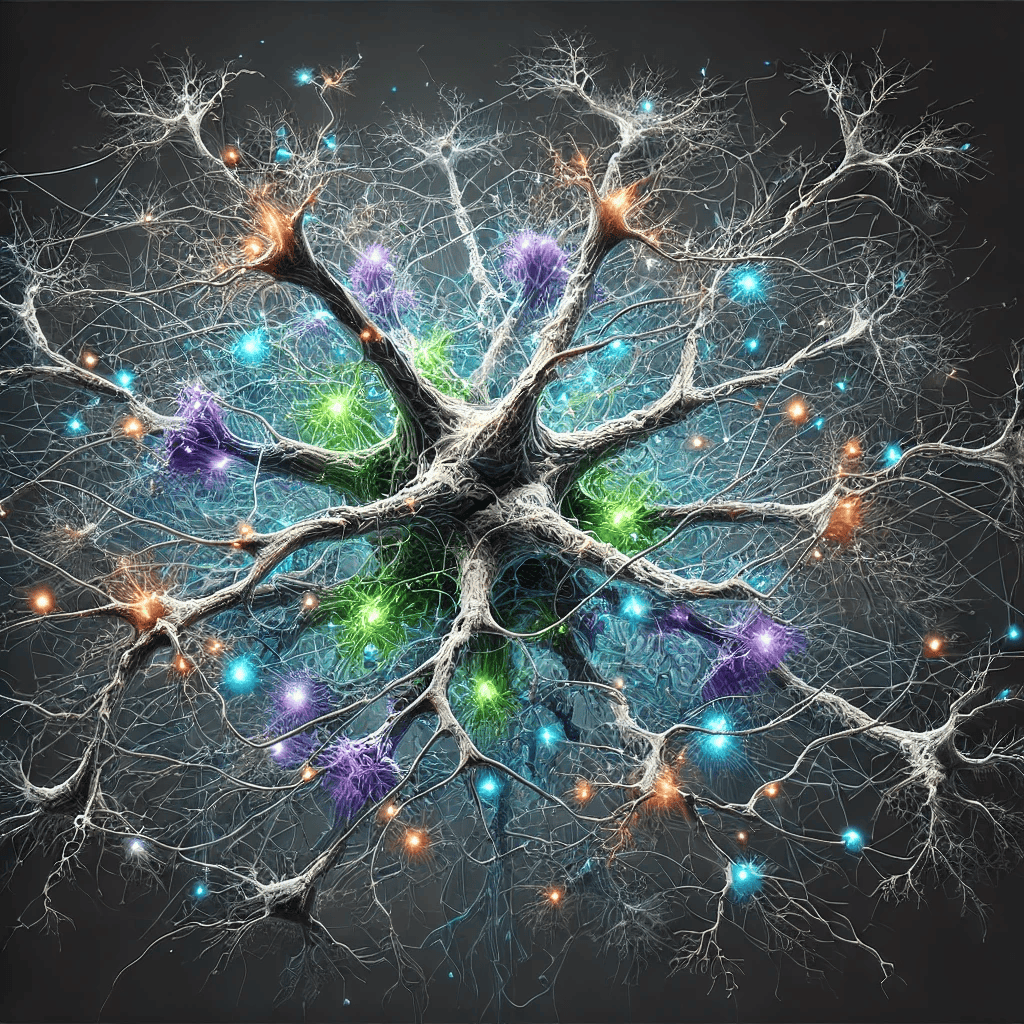
\includegraphics[width=0.8\textwidth]{neuropil.png}

    \caption{The neuropil is the most tangled layer of the cortical sheet}
\end{figure}

To model energetic coherence in the neuropil, we can employ the Jacobian of the stress-energy tensor with specific coupling terms that capture interactions between different components:

$\partial_\sigma T_{\mu\nu}(x) = \sum_i J_i(x) + \sum_{j,k} C_{jk}(x)$

\text{Where:}
\begin{itemize}
\item $T_{\mu\nu}$ represents the stress-energy tensor for the neuropil
\item $J_i$ captures local energy flows within specific components
\item $C_{jk}$ represents coupling terms between different elements
\item $x$ denotes position within the neuropil space
\end{itemize}

This organization creates the conditions necessary for sustained coherent states through the precise balance of energy flows across multiple scales \cite{Mishchenko2010}. When we examine the temporal evolution of these states, we can represent the dynamics using a modified form of the stress-energy tensor's Jacobian that incorporates both spatial and temporal derivatives:

$\partial_\sigma\partial_\tau T_{\mu\nu} = \sum_i \partial_\sigma J_i + \sum_{j,k} \partial_\tau C_{jk} + I_{\mu\nu}$

\text{Where:}
\begin{itemize}
\item $\partial_\sigma\partial_\tau$ represents the spatiotemporal evolution
\item $I_{\mu\nu}$ captures interface terms between adjacent regions
\end{itemize}

The interface terms are particularly important for understanding how coherent states propagate through the neuropil \cite{Doron2017}. These terms must satisfy certain continuity conditions:

$I_{\mu\nu}|_{\text{boundary}} = \text{continuous across regions}$

This constraint ensures smooth transitions between adjacent domains while maintaining global coherence. The neuropil's structure supports these transitions through specific biophysical mechanisms and architectural organization \cite{Korogod2015}.

1. Local Field Dynamics:

$\nabla \cdot \mathbf{E} = \frac{\rho}{\varepsilon}$

\text{Where:}
\begin{itemize}
\item $\mathbf{E}$ represents local field strength
\item $\rho$ captures charge density
\item $\varepsilon$ reflects local permittivity \cite{Savtchenko2014}
\end{itemize}

2. Wave Propagation:

$(\nabla^2 - \frac{1}{v^2}\frac{\partial^2}{\partial t^2})\psi = 0$

\text{Where:}
\begin{itemize}
\item $\psi$ represents the wave function
\item $v$ is the propagation velocity in the medium \cite{Arbib1998}
\end{itemize}

These equations describe how the neuropil supports both standing waves and propagating disturbances while maintaining coherent states. The solution space is constrained by the physical properties of the neuropil \cite{Peters1991}.

These constraints help ensure that energy flows remain within bounds that support conscious processing while allowing for dynamic responses to changing conditions \cite{Sorra2000}. The neuropil thus emerges as the critical substrate for implementing ECC's principles, providing both the physical structure and dynamic properties necessary for maintaining coherent conscious states.

\begin{figure}[h]
    \centering
    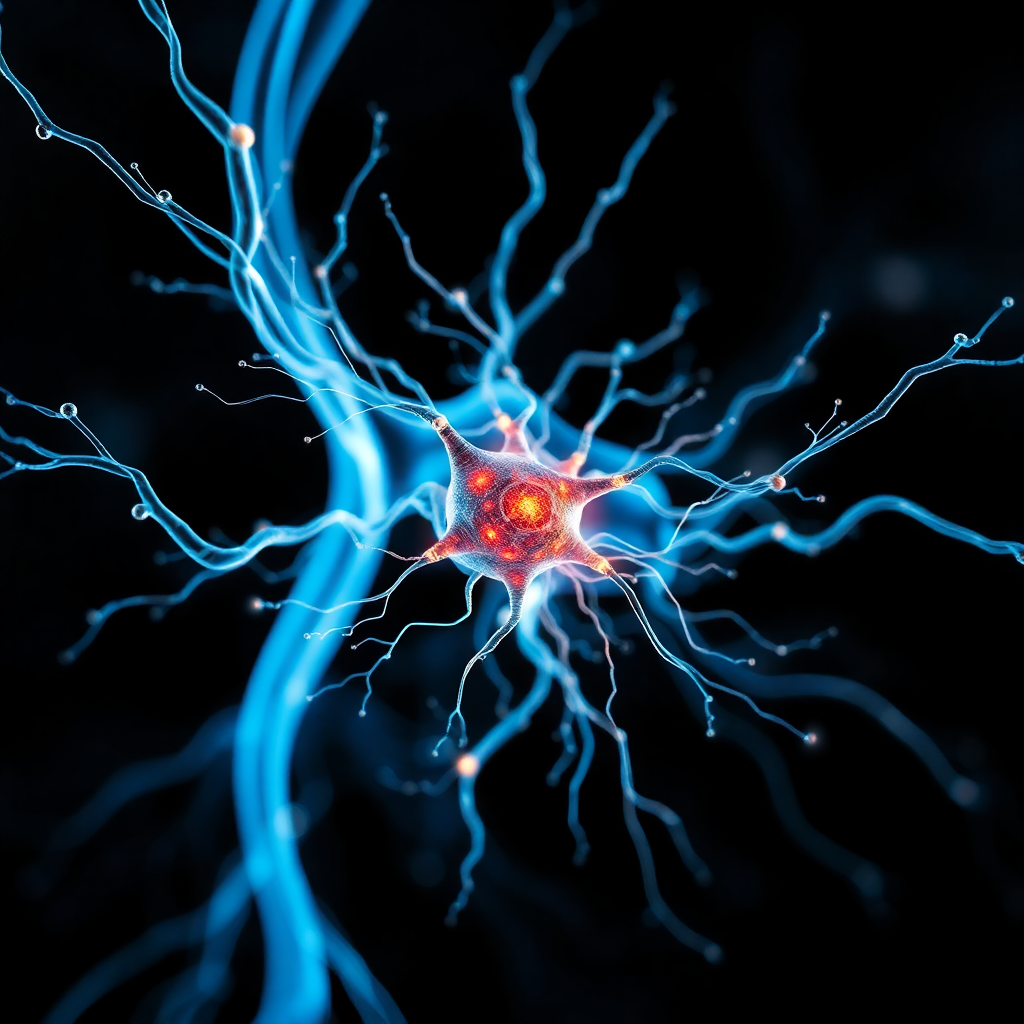
\includegraphics[width=0.8\textwidth]{images/neuropil2.png}

    \caption{Typical neuron of the neuropil.}
\end{figure}

The neuropil represents a critical domain for understanding how conscious states emerge from neural organization, as it provides the physical substrate where energetic coherence manifests at multiple scales \cite{Ventura1999}. This dense mesh of neural processes, glial extensions, and extracellular matrix creates the conditions necessary for maintaining coherent energy states while enabling dynamic information processing. Understanding how these components interact within the neuropil proves essential for any complete theory of consciousness.

The significance of neuropil organization extends beyond traditional connectionist approaches that focus primarily on synaptic connections between neurons \cite{Kasthuri2015}. Within this intricate space, multiple modes of communication operate simultaneously, including volume transmission, ephaptic coupling, and field effects that influence neural activity through non-synaptic mechanisms. These various forms of interaction create a rich landscape of possible states that supports both local processing and global integration of neural activity.

The physical properties of the neuropil prove particularly crucial for maintaining energetic coherence \cite{Korogod2015}. Its precise spatial organization enables the establishment of stable field patterns while allowing for rapid reconfiguration based on computational demands. The density and arrangement of cellular processes within the neuropil create conditions that support wave propagation while maintaining boundaries between different functional domains \cite{Arbib1998}. This balanced organization enables both segregation and integration of neural processing.

Astrocytic processes within the neuropil play an especially important role in maintaining coherent states \cite{Ventura1999}. Their extensive branching patterns and strategic positioning allow them to monitor and modulate synaptic activity while maintaining ion homeostasis across substantial volumes of tissue. The three-dimensional organization of astrocytic processes creates a continuous network that can coordinate energy distribution and maintain stable background conditions necessary for conscious processing.

The extracellular space within the neuropil, far from being a simple gap between cells, represents a highly structured environment that shapes both molecular diffusion and field effects \cite{Savtchenko2014}. The precise arrangement of extracellular matrix components influences how signals propagate through this space, affecting both local interactions and longer-range coordination. This structured environment proves essential for maintaining the specific patterns of energy flow that support conscious states.

The dynamic nature of neuropil organization deserves particular attention \cite{Sorra2000}. Rather than representing a static structure, the neuropil continuously adapts its properties in response to neural activity and metabolic demands. This adaptability enables sophisticated regulation of energy distribution and information processing while maintaining the stability necessary for coherent conscious experience. Understanding these dynamics proves crucial for developing accurate models of how consciousness emerges from neural activity.

Moreover, the neuropil's organization reflects evolutionary optimization for both information processing efficiency and energy management \cite{Peters1991}. The precise arrangement of cellular processes minimizes wiring length while maximizing computational capacity, creating conditions that support conscious processing while respecting metabolic constraints. This efficiency proves essential for maintaining coherent states across extended periods without excessive energy expenditure.

These considerations reveal why detailed modeling of neuropil organization and dynamics proves essential for understanding consciousness \cite{Mishchenko2010}. The emergence of coherent conscious states depends critically on the specific properties and interactions that occur within this complex domain. Any complete theory of consciousness must account for how the neuropil's structure enables both local processing and global integration while maintaining energetic efficiency.

The challenge of modeling neuropil dynamics reflects deeper questions about how consciousness emerges from biological organization \cite{Denk2004}. Traditional computational approaches, focused primarily on discrete neuronal interactions, fail to capture the continuous, field-like properties that arise from the neuropil's intricate structure. New mathematical frameworks must be developed that can represent both the discrete and continuous aspects of neural processing while accounting for the multiple scales of organization present in neural tissue.

The integration of various modeling approaches becomes particularly crucial when considering the neuropil's role in conscious processing \cite{Haehn2014}. Field theories must be combined with detailed cellular models, while accounting for the structured diffusion processes that occur in the extracellular space. These different perspectives must be unified through mathematical frameworks that can capture both the local dynamics of individual components and the emergent properties that arise from their collective interaction.

Perhaps most significantly, neuropil modeling reveals fundamental principles about how biological systems achieve conscious processing \cite{Helmstaedter2013}. The sophisticated organization of the neuropil, with its multiple overlapping domains of interaction and regulation, demonstrates how complex conscious states can emerge from physical processes while maintaining both stability and adaptability. This understanding proves essential for both theoretical developments in consciousness studies and practical applications in treating neurological disorders.

The implications extend beyond neuroscience to influence our broader understanding of consciousness itself \cite{White1986}. The neuropil's organization suggests that consciousness requires specific forms of physical implementation that support both local processing and global integration through continuous field-like interactions. This perspective challenges purely computational approaches to consciousness while suggesting new directions for developing artificial systems that might support conscious-like processing.